\documentclass[a4paper]{article}
\usepackage{amsmath}
\usepackage{amsthm}
\usepackage{amsfonts}
\usepackage{mathtools}
\newtheorem{thm}{Theorem}
\usepackage[english]{babel}
\usepackage[utf8]{inputenc}
\usepackage{graphicx}
\usepackage[colorinlistoftodos]{todonotes}

\title{Notes on Elliptic Curve Operation}

\author{}

\date{}
\begin{document}
\maketitle

% \begin{abstract}
% This paper will state and prove the quadratic formula.
% \end{abstract}

\section{Introduction}
which 

\section{Twisted Edwards Curves}

The \textit{characteristic} of a field $F$ is the smallest positive integer $m$ such that
$$\underbrace{1+1+...+1}_{m}$$
denoted as $char(F)=m$
If no such $m$ exists then the field is said to have characteristic 0. The characteristic of any field is
either 0 or a prime $p$.

If $F$ is a finite field of characteristic $p$, then the \textit{order} of $F$ is a prime power $q=p^r$ for some positive integer $r$, and we write $F = \mathbb{F}_{p^r}$ or $F = \mathbb{F}_q$. \\

Fix a field $k$ with char($k$) $\neq 2$ \footnote{The \textit{characteristic} of a field is the smallest positive integer $m$ such that $\underbrace{1+1+...+1}_{m}=0$}. Fix distinct nonzero elements $a,d \in k$. The twisted Edwards curve with coefficients $a$ and $d$ is the curve
$$E_{E,a,d}:ax^2+y^2=1+dx^2y^2.$$
The elliptic curve has $j$-invariant $16(a^2+14ad+d^2)^3/ad(a-d)^4$.
\begin{description}
\item[Addition formulae.] Let $(x_1,y_1),(x_2,y_2)$ be points on the twisted Edwards curve $E_{E,a,d}:ax^2+y^2=1+dx^2y^2$. The sum of these points on $E_{E,a,d}$ is
$$(x_1,y_1)+(x_2,y_2)=\left(\frac{x_1y_2+y_1x_2}{1+dx_1x_2y_1y_2},\frac{y_1y_2-ax_1x_2}{1-dx_1x_2y_1y_2} \right).$$
The neutral element is $(0,1)$, and the negative of $(x_1,y_1)$ is $(-x_1,y_1)$.
\end{description}

\begin{description}
\item[Doubling formulae.] Doublinh can be performed with exactly the same formula as addition. Doublong of a point $(x_1,y_1)$ on the curve $E_{E,a,d}$ is:
$$(x_3,y_3)=\left(\frac{2x_1y_1}{ax_1^2+y_1^2},\frac{y_1^2-ax_1^2}{2-ax_1^2-y_1^2} \right)$$

\end{description}

% \begin{description}
% \item[Affine addition formulae (independent of $d$)] 
% After straight forward eliminations, we can express $a$ and $d$ in terms of $x_1,x_2,y_1,y_2$. The addition formulae are then as follows,
% $$(x_1,y_1)+(x_2,y_2)=\left(\frac{x_1y_1+x_2y_2}{y_1y_2+ax_1x_2},\frac{x_1y_1-x_2y_2}{x_1y_2-y_1x_2} \right)=(x_3,y_3)$$
% \end{description}
% However, these formulae fail for point doubling. In addition, there are exceptional cases even if $d$ is not a square in $K$ and $a$ is a square in $K$. The following theorem states these points explicitly.

% \begin{description}
% \item[Affine doubling formulae (independent of $d$)] 
% $$ 2(x_1,y_1)= \left(\frac{2x_1y_1}{{y_1}^2+a{x_1}^2},\frac{{y_1}^2-a{x_1}^2}{2-{y_1}^2-a{x_1}^2}\right) = (x_3,y_3)$$
% \end{description}


% \begin{description}
% \item[Theorem 1]
% Let $K$ be a field of odd characteristic. Let $E_{E,a,d}$ be a twisted Edwards curve defined over $K$. Let $P=(x_1,y_1)$ and $Q=(x_2,y_2)$ be points on $E_{E,a,d}$. Assume that $P$ is fixed.

% If $x_1=0$ or $y_1=0$ then $y_1y_2+ax_1x_2=0$ if and only if $Q in S_x$ where $S_x=\{(y_1/\sqrt{a},-x_1\sqrt{a}),(-y_1/\sqrt{a},x_1\sqrt{a})\}$.

% Similarly, $x_1y_2-y_1x_2=0$ if and only if $Q in S_y$ where $S_y=\{(x_1,y_1),(-x_1,-y_1)\}$.

% Otherwise (i.e. $x_1 \neq 0$ and $y_1\neq 0$), $S_x$ and $S_y$ are given by
% $$S_x=\left\{\left(\frac{y_1}{\sqrt{a}},-x_1\sqrt{a}\right),\left(-\frac{y_1}{\sqrt{a}},x_1\sqrt{a}\right),\left(\frac{1}{x_1\sqrt{ad}},-\frac{\sqrt{a}}{y_1\sqrt{d}}\right),\left(-\frac{1}{x_1\sqrt{ad}},\frac{\sqrt{a}}{y_1\sqrt{d}}\right)\right\},$$
% $$S_y=\left\{(x_1,y_1),(-x_1,-y_1),\left(\frac{1}{y_1\sqrt{d}},\frac{1}{x_1\sqrt{d}}\right),\left(-\frac{1}{y_1\sqrt{d}},-\frac{1}{x_1\sqrt{d}}\right)\right\}.$$


% \end{description}

\section{Projective Twisted Edwards Coordinates}
According to Bernstein et al.\cite{hisil2008twisted}, we can work on the projective twisted Edwards curve to avoid inversions.
$$(aX^2+Y^2)Z^2=Z^4+dX^2Y^2.$$
For $Z_1 \neq 0$ the homogeneous point $(X_1:Y_1:Z_1)$ represents the affine point $(X_1/Z_1,Y_1/Z_1)$ on $E_{E,a,d}$.
\begin{description}
\item[Addition in Projective Twisted Coordinates.]
The following formulas compute $(X_3:Y_3:Z_3)=(X_1:Y_1:Z_1)+(X_2:Y_2:Z_2)$ in $9M+1S+2D+7add$, where the 2D are one multiplication by $a$ and one by $d$:

\begin{align*}
A & =Z_1\cdot Z_2; \\
B & =dA^2;\\
C & =X_1\cdot X_2; \\
D & =Y_1\cdot Y_2; \\
E & =C\cdot D;\\
H & =C-aD;\\
I & =(X_1+Y_1)\cdot (X_2+Y_2)-C-D;\\
X_3 & =(E+B)\cdot H;\\
Y_3 & =(E-B)\cdot I;\\
Z_3 & =A\cdot H\cdot I.
\end{align*}

\end{description}

\begin{description}
\item[Doubling in Projective Twisted Coordinates.]
The following formulas compute $(X_3:Y_3:Z_3)=2(X_1:Y_1:Z_1)$ in $3M+4S+2D+6add$, where the 2D are pme multiplication by $a$ and one by $2d$:
\begin{align*}
    A & =X_1^2; \\
    B & =Y_1^2;U=aB;\\
    C & =A+U;\\
    D & =A-U;\\
    E & =(X_1+Y_1)^2-A-B;\\
    X_3 & =C\cdot D;\\
    Y_3 & =E\cdot (C-2dZ_1^2);\\
    Z_3 & =D\cdot E
\end{align*}

\end{description}


\section{JubJub}
% https://z.cash/technology/jubjub.html
Jubjub is a twisted Edwards curve of the form 
$$-x^2+y^2=1+dx^2y^2$$
built over the BLS12-381 scalar field, with $d=-\frac{10240}{10241}$. It has a complete addition law that avoids edge cases with doubling and identities, making it convenient to work with inside of an arithmetic circuit.
$$(x_1,y_1)+(x_2,y_2)=\left(\frac{x_1y_2+y_1x_2}{1+dx_1x_2y_1y_2},\frac{y_1y_2+x_1x_2}{1-dx_1x_2y_1y_2} \right).$$


% \end{document}

% \section{Introduction}

% We have all, at some point, learned the quadratic formula. Usually, we learn how to use it to find solutions of a quadratic equation. We might have seen the proof at this point, but most of us did not commit it to memory since the proof does not help us to use the formula.

% \section{The Quadratic Formula}
% \label{sec:examples}

% \begin{thm} Let a, b, and c be real number. The solutions of $ax^2+bx+c=0$ are 
% $$x=\frac{-b\pm \sqrt{b^2-4ac}}{2a}.$$
% %\begin{array}${*{20}c}{x = \frac{{ - b \pm \sqrt {b^2 - 4ac} }}{{2a}}} & {{\rm{when}}} & {ax^2 + bx + c = 0}$ \\ \end{array}

% \end{thm}

% \begin{proof} In order to prove the quadratic formula, we use the process of completing the square. Starting with $ax^2+bx+c=c$, arithmetic gives 
% \begin{align*} 
% \\ax^2+bx&=-c,
% \\x^2+\frac{b}{a}x&=-\frac{c}{a},
% \\x^2+\frac{b}{a}x+\frac{b^2}{4a^2}&=-\frac{c}{a}+\frac{b^2}{4a^2},
% \\\Bigg(x+\frac{b}{2a}\Bigg)^2&=-\frac{4ac}{4a^2}+\frac{b^2}{4a^2},
% \\x+\frac{b}{2a}&=\pm\sqrt[]{\frac{b-4ac}{4a^2}}
% \\x&=\frac{-b\pm\sqrt[]{b^2-4ac}}{2a}
% \end{align*}
% \end{proof}
% % \end{document}


% Theorem 1

% Comments can be added to the margins of the document using the \todo{Here's a comment in the margin!} todo command, as shown in the example on the right. You can also add inline comments:

% \todo[inline, color=green!40]{This is an inline comment.}

% \subsection{How to Include Figures}

% First you have to upload the image file (JPEG, PNG or PDF) from your computer to writeLaTeX using the upload link the project menu. Then use the includegraphics command to include it in your document. Use the figure environment and the caption command to add a number and a caption to your figure. See the code for Figure \ref{fig:frog} in this section for an example.

% \begin{figure}
% \centering
% 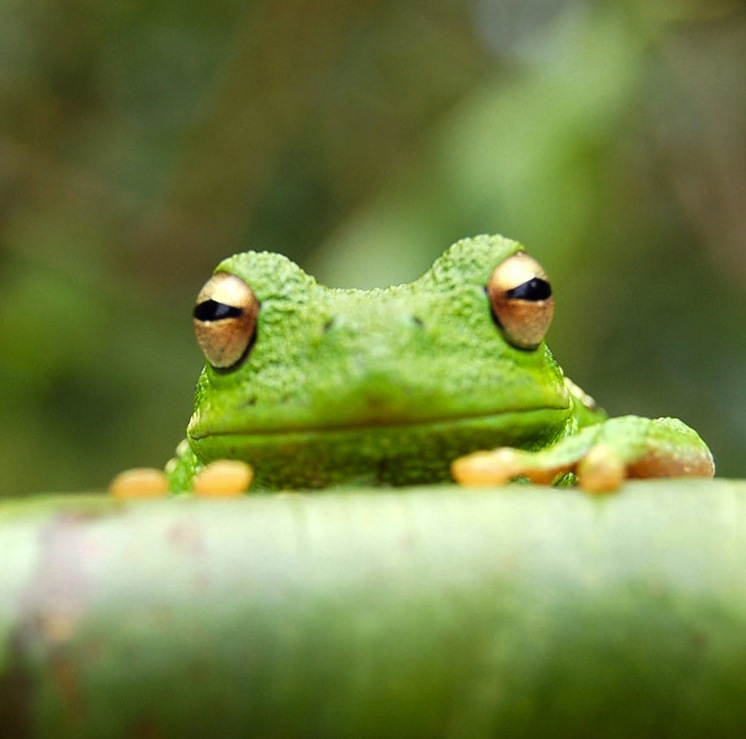
\includegraphics[width=0.3\textwidth]{frog.jpg}
% \caption{\label{fig:frog}This frog was uploaded to writeLaTeX via the project menu.}
% \end{figure}

% \subsection{How to Make Tables}

% Use the table and tabular commands for basic tables --- see Table~\ref{tab:widgets}, for example.

% \begin{table}
% \centering
% \begin{tabular}{l|r}
% Item & Quantity \\\hline
% Widgets & 42 \\
% Gadgets & 13
% \end{tabular}
% \caption{\label{tab:widgets}An example table.}
% \end{table}

% \subsection{How to Write Mathematics}

% \LaTeX{} is great at typesetting mathematics. Let $X_1, X_2, \ldots, X_n$ be a sequence of independent and identically distributed random variables with $\text{E}[X_i] = \mu$ and $\text{Var}[X_i] = \sigma^2 < \infty$, and let
% $$S_n = \frac{X_1 + X_2 + \cdots + X_n}{n}
%       = \frac{1}{n}\sum_{i}^{n} X_i$$
% denote their mean. Then as $n$ approaches infinity, the random variables $\sqrt{n}(S_n - \mu)$ converge in distribution to a normal $\mathcal{N}(0, \sigma^2)$.

% \subsection{How to Make Sections and Subsections}

% Use section and subsection commands to organize your document. \LaTeX{} handles all the formatting and numbering automatically. Use ref and label commands for cross-references.

% \subsection{How to Make Lists}

% You can make lists with automatic numbering \dots

% \begin{enumerate}
% \item Like this,
% \item and like this.
% \end{enumerate}
% \dots or bullet points \dots
% \begin{itemize}
% \item Like this,
% \item and like this.
% \end{itemize}
% \dots or with words and descriptions \dots
% \begin{description}
% \item[Word] Definition
% \item[Concept] Explanation
% \item[Idea] Text
% \end{description}

% We hope you find write\LaTeX\ useful, and please let us know if you have any feedback using the help menu above.
\bibliographystyle{plain}
\bibliography{ecc}

\end{document}